\documentclass[11pt]{article}

\usepackage[]{fontenc}
\usepackage[latin1]{inputenc}
\usepackage[english]{babel}
\usepackage{graphicx}
\usepackage{color}
%\usepackage{url}
%\usepackage{pt8hyph}
%\renewcommand\url{\begingroup\urlstyle{sf}\Url}


%%%% Du kannst
\newcommand{\commentary}[1]{\textsl{\small[\textbf{comment:} #1]}}
%\newcommand{\commentary}[1]{}



\begin{document}

% The Title
\begin{center}

{\large
{\sc Christian-Albrechts-Universit\"{a}t zu Kiel} \\
Institut f\"{u}r Informatik und Praktische Mathematik \\
Lehrstuhl f\"{u}r Software-Technologie }

\bigskip

{\Large\it Concept for the Testing Framework of the CoMa Project}

\bigskip

{\small Oliver Niemann} \\
{\small Olle Nebendahl} \\
{\small Thiago Tonelli Bartolomei}

\end{center}

%-----------------------------------------------
%-----------------------------------------------
\section{Introduction}

\indent

\commentary{ms: Ich verbessere kein Englisch, bis auf Notf"alle}

CoMa, short for ``Conference Manager'', is a development project that aims
to produce an automated conference manager. The participants were divided
in four groups. One group will develop the conference manager using the
Java language while other two will use the Php language. All groups share
the same specification and the same Data Model, with minor changes. The
last group is responsible for testing the implementations and guarantee the
functionalities described in the specification. This document describes the
concept developed for testing the implementations of the CoMa project.
\commentary{ms: ok}

%-----------------------------------------------
%-----------------------------------------------
\section{Tests Specification}

\indent

This section describes the tests that are going to be performed. The next subsection details the architecture model the groups are going to use to implement CoMa. The subsequent subsections describe the tests that will be performed for each part of these architectures. The last subsection details how test results will be presented.

%-----------------------------------------------
\subsection{Architecture Model}

\indent

There are several diferent models for the architecture design. We assume that the groups are going to use something similar to a 3-tier Architecture. In a 3-tier architecture, the application is divided in ``View'', ``Business'' and ``Data''. The modules implementing each tier should be as separated and independent from each other as possible. When independency is achieved, one is able to reuse code, for example changing the View module, but keeping the Business and Data modules. Such an approach is represented in Figure~\ref{fig:3tier}.



\begin{figure}[htbp]
  \centering
  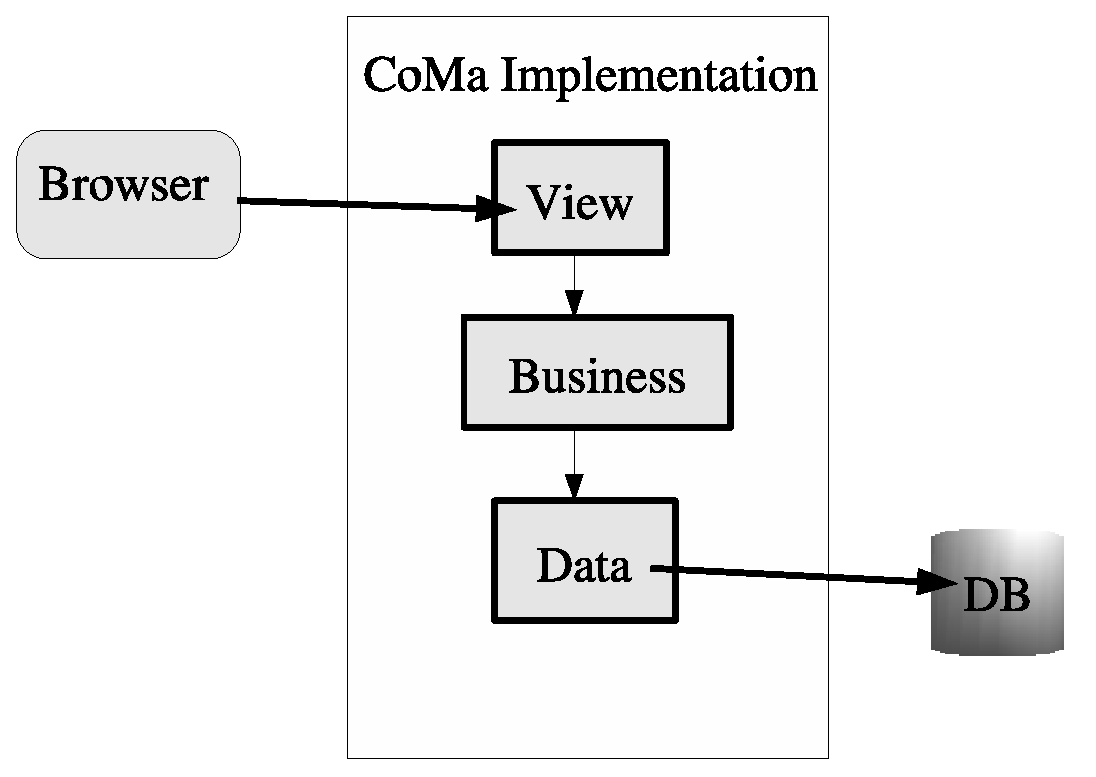
\includegraphics[width=8cm]{3tier}
  \caption{The 3-tier Architecture}
  \label{fig:3tier}
\end{figure}


The View tier is responsible only for user presentation and interaction. It means that in this tier the application should not have any business rules. It is only the external representation of the application data and state, as well as presenting the user means for interaction with the business tier.

The Business tier performs the application logic, defining ``what'' the application is meant to do. This tier protects the direct use of data by the user, and provides the correct ways of accessing it.

The Data tier is responsible for maintaining all the Data needed by the application, ``data persistence'' in short. This tier is usually a relational database and the modules needed to correctly access the database.

This logical separation of concearns allow us to design tests that are specific for each tier. The tests designed for one tier are independent from other tiers.

The next subsections present the tests that will be performed on each tier, separating them in Automated Tests, that are executed automaticaly using scripts or special tools, and Manual Tests, that are performed manually by the testers.

%-----------------------------------------------
\subsection{Data Tests}

\indent

The Data tier can be totaly checked using Automated Tests.

\subsubsection*{Database Consistency Checks}

\indent

The Entity Relationship Diagram describes the structure of the Data stored in the Database. But it doens't say anything about the semantic rules of this Data. For example, a table called {\it Student} with a field called {\it Note} can describe that the {\it Note} is an Integer, but cannot say what a value {\it 1} in this field means. For this reason, Database Consistency Checks must be performed, to be sure that the Data has semantic consistency.

To check the consistency, check scripts are going to be implemented. Since each implementation has its own semantic, 3 different scripts must be developed. In order to know exactly the semantic that the scripts check, a {\it Data Specification Document} must be written by each group.

These tests are tied to the Use Case Driven Test Cases described in the next subsection. The consistency check scripts check if the Database is consistent in a determined moment in time. So, we can run the consistency check before and after each use case is performed, in order to check if this use case affects semantic consistency.

%-----------------------------------------------
\subsection{Business Tests}

\indent

The Business tier can be totaly checked using Automated Tests.

\subsubsection*{Compilation Tests}

\indent

Since Php is not compiled until running time, this section applies only for the Java implementation.

\textcolor{red}{Are we going to do these tests in Java?? Is it necessary now?}

\commentary{The testers have provided an ant-file. It should be compilable
  (they say so, even on the solaris machines and on other platforms). I
  (Martin) reported some time ago some compile-errors, because the
  ant-build file did not work. My opinion is: that sure one should test
  that (but after that's tested it's self-evident, that compilability
  should maintained by the group from that point on.}

\subsubsection*{Use Case Driven Test Cases}

\indent

\textcolor{red}{I am not sure if it is true now, since I couldn't compile
  these tex files to check if somebody followed some specification or not.
  Anyway, I assume each has its own... not?}

\commentary{ms: then complain! I complained some time ago that I could not
  tex their stuff. The said: well, it's not so important. If it's important
  for you to read their stuff, they must provided you with a viewable
  document. I would say, if they choose \TeX\ (which is quite portable and
  a good choice for platform independant documentation), they should not
  use 15 esoteric packages that only one person in the world has, namely
  they.}

Despite of having a similar \textit{Informal Requirements Document}, each
group has a separated {\it Specification Document}. This documents describe
in detail all the functionality of the system. From these documents, use
cases can be derived and test scripts written. The reach of these scripts
are still dependant on the quality of the Testing Frameworks we will be
able to install.

These tests have two main purposes. First, they assure that all the functionality described in the specification document is available and works properly. Sencond, they check if the application is prepared to deal extreme and special cases, like non-conforming use input, sql-injection attacks and Database inconsistency.

\subsubsection*{Unit Tests}

\indent

\textcolor{red}{I am not sure about the efectiveness and importance of creating unit tests now. I think the great importance would be for ``Change Management''}

{\it Unit Tests}s are simple tests made to check a low level function of a system. Usually the programmers themselves write unit tests for the funtions or methods they develop, to make sure that, in every case, they respond something meanfull. 

Another important factor of {\it Unit Tests} is the support for {\it Change Management}. A battery of {\it Unit Tests} can be develop to check most, preferably all, the functions of a system. When a new Feature is created or deployed, this battery can be run to check the effects of this new module, what guarantees that it didn't disturb other parts of the system.

The creation of the {\it Unit Tests} is planned but should be of lower priority, since they required the testers to understand the code deeply, what could require to much time and effort.

\subsubsection*{E-Mail Tests}

\indent

\textcolor{red}{Again, not sure if we should do this}

Some functions include sending emails. To test these funtions an email account must be created and then a script can be developed to check if the emails are been correctly sent.


%-----------------------------------------------
\subsection{View Tests}

\indent

\subsubsection{Automated Tests}

\subsubsection*{W3C Conformance}

\indent

To check if every page in the system is W3C conformant, a W3C Html Validator is going to be used. The Validator is an application that receives a link to the web page and checks its conformity, generating a log in Html.

In order to guarantee that all the pages are checked, the validator must be called after each use case, validating the result of its actions.

\subsubsection{Manual Tests}

\subsubsection*{Browser Compatibility and Display}

\indent

Browser compatibility checks cannot be done in an automated way, since we cannot forsee how each browser will interpretate the page. For this reason, each use case will have to be executed manually in each Browser, and the Tester will then check if the result was as expected. Furthermore, 

There are tests planned for the following Brosers:

\begin{itemize}

\item Firefox 1.0
\item Internet Explorer XX
\item Opera XX

\end{itemize}

%-----------------------------------------------
\subsection{General Tests}

\indent 

Some general automated tests.

\subsubsection*{Performance}

\indent

\textcolor{red}{are we going to check performance??}

\commentary{ms: difficult. I'd say no, at least no in particular. If one
  sees that perfomance is low, one can report that, though.}


%-----------------------------------------------
%-----------------------------------------------
\section{Test Results Presentation}

\indent

\textcolor{red}{I think we should write scripts that write html pages,
so that everybody can check if their systems are working directly from
a website.. snert in this case..}

\end{document}
